\chapter{Detalles de Implementación}\label{chapter:implementation}

Para la validación de la propuesta planteada a partir del esquema general de definición de los datos de entrada se concibió 
un prototipo de sistema. Este implementa los modelos de generación para el fútbol y el boxeo y permite la interacción
 con los mismos. Para facilitar la interacción se implementó a su vez una interfaz gráfica sencilla. A continuación se presentan 
 detalles generales del sistema, funciones de interés y una presentación de la interfaz creada. Se utilizó \emph{python} como 
 lenguaje de programación.
 
\section{Detalles generales del sistema}

\begin{figure}[!]
    \begin{center}
        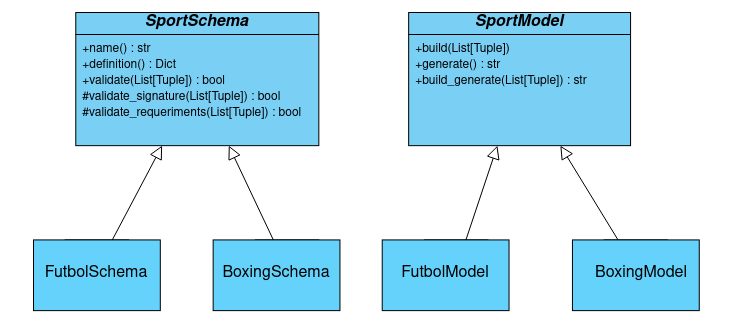
\includegraphics[width=\textwidth]{Graphics/classDef3.png}
    \end{center}
    \caption{Definición de las clases principales}
    \label{fig_classDef}
\end{figure}

Para la representación de los esquemas y de los modelos se crearon dos clases abstractas, \textit{SportSchema} y 
\textit{SportModel}. En la figura (\ref{fig_classDef}) se representan cada una con la signatura principal. 

Los esquemas, con el m\'etodo \emph{validate\_signature}, validan la entrada en cuanto a su signatura, o sea, comprueban que 
su representación en cada uno de los valores se corresponda con la definición. La \textit{definición} (m\'etodo \emph{definition}) 
de un esquema es el conjunto de valores admitidos por cada tipo principal (los tipos principales son los definidos en el 
meta esquema general). A su vez, el método \emph{validate\_requeriments} se utiliza para validar si en el conjunto de entrada
 existe un conjunto minimal de los datos a partir de los cuales es posible la generación de texto. El m\'etodo \emph{name} devuelve 
 un nombre identificativo del esquema, debe ser único. La funcionalidad de \emph{validate} es una conjunción de los otros dos 
 métodos de validación. 




Los modelos para su correcto funcionamiento dependen de un primer llamado al método \emph{build} previo a cualquier 
secuencia de \emph{generate}. El método \emph{build} de los modelos es el que se encarga de procesar la entrada, hacer las 
transformaciones correspondientes de los datos. Durante su ejecución, los modelos completan toda la información 
necesaria para las distintas etapas de generación del texto que se definan. Para esto, se definen estructuras propias de cada 
modelo para representar la información. Con el uso de la información estructurada e interpretada en la construcción del modelo, 
con el método \emph{generate} se generan las distintas piezas textuales que conforman el reporte. El m\'etodo \emph{build\_generate} 
unifica un llamado a \emph{build} seguido de uno a \emph{generate}.

%Los modelos en build tienen que hacer todo el proceso de procesamiento de los datos, llenando tomados
%las variables y estructuras que son necesarias para generar el texto en cada una de las etapas. Luego
%en generate los modelos van en base a la representación interna de los datos, generando el texto de 
%caa una de las piezas comunicativas.

\begin{figure}[!]
    \begin{center}
        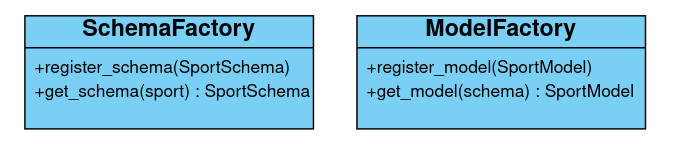
\includegraphics[width=\textwidth]{Graphics/factories.png}
    \end{center}
    \caption{Definición de las clases \emph{Factory}}
    \label{fig_classFactory}
\end{figure}


El flujo principal del programa se encuentra representado en el \textit{Algoritmo Principal} a continuación. Se utilizó el patrón 
\emph{Factory} (de Factoría, en español) para la selección de los modelos y los esquemas (Ver fig\ref{fig_classFactory}). 
Se planteó de esta forma, ya que el prototipo podría adaptarse más fácilmente a nuevos modelos y esquemas sin necesidad de grandes 
cambios en el código. %Las clases \textit{SchemaFactory} y \textit{ModelFactory}

\pagebreak

\begin{verbatim}
Algoritmo principal

  Entrada: knowdlage_tuple:List[Tuple], selected_sport
  Salida : str

    schema = schema_factory.get_schema(selected_sport)
    if not schema.validate(knowdlage_tuple):
        mostrar error
        FIN
    model = model_factory.get_model(schema)
    summary = model.build_generate(knowdlage_tuple)
    return summary

\end{verbatim}



\section{Sistema de plantillas}


Para el llenado de la plantilla se utiliza la función select template, que a su vez emplea la función
fille template  y genre desambiguation.

La función  select template recibe el conjunto de posibles plantillas a emplear en la situación así como un 
diccionario de representación, donde las llaves constituyen las ranuras en las plantillas y los valores, el Valor
de ese dato en el contexto.

Como el sistema propuesto presenta cierto grado de sensibilidad ante la ausencia de datos, es posible
que haya plantillas en el conjunto para la que alguna de sus ranuras no tiene valor. Para esto, el algoritmo
selecciona automáticamente una plantilla del conjunto, si en el diccionario todas las ranuras tienen un valor 
correspondiente se selecciona, si no, se descarta y se repite el proceso. Siempre se garantiza que habrá
al menos una plantilla en el conjunto que funcione, porque presentará el subconjunto minimal de datos que
admite el sistema en ese contexto. La plantilla seleccionada se rellena utilizando el  método fill template
que sustituye las ranuras de la plantilla por el valor real.

%##1





\section{Interfaz gráfica}


%##2

Para poder trabajar más fácil con la propuesta, se proporcionó una interfaz gáfica. Esta interfaz es sencilla
 y se concibió utilizando el framework de python streamlit. Se da la opción a los usuarios de aportar
 datos en forma de archivos, ya sea a partir de definir la ruta local o cargando directamente el archivo.

 Para permitir  esta interacción se concibió una estructura intermedia para poder representar las tuplas
 de entrada en base a archivos json.  Cada tupla se concibe de la forma "id"

 donde cada valor representa el valor de la tupla............. en esa posición. Si no se proporciona uno de los 
 valores, esa posición se considera vacía. Ejemplo de representación se puede ver en imagen.

 Desde la primera interfaz se puede interactuar con el conjunto de datos de prueba que se concibieron
junto a la propuesta. Para ello hay que seleccionar el deporte deseado y uno entre los eventos de prueba.
El sistema mostrará el texto producido en pantalla, luego de presionar el botón "generar".


 




%##3






